\chapter{Experiments on Real Networks}

Networks collected from real world data are often used as a proving ground for community detection methods. Rather than rely on communities being assigned by the model generating the network, community structure is taken from \textit{metadata}, observed information about the network outside of its structural information. This metadata can be taken from observed interactions of individuals, membership of a particular group on a social network, or behavior patterns.  It should be noted that the assumption that the metadata represents the true community structure is not always warranted. The common, small scale networks typically used in benchmarking and comparison may not give the full picture of an algorithms behaviors, so it is critical that more robust testing must be done. In these tests, the goal is to show that the algorithms do indeed extract a coherent community structure comparable to to other methods.


\begin{table}[h!]
	\centering
	\begin{tabular}{ |l | l| l | l | } 
		\hline
		\multicolumn{1}{|c|}{\textbf{Network}} & \multicolumn{1}{|c|}{\textbf{Nodes}} &
		\multicolumn{1}{|c|}{\textbf{Edges}} & \multicolumn{1}{|c|}{\textbf{True Communities (Metadata)}} \\
		\hline
		\hline
		Zachary's Karate Club & 34  & 78 & 2\\ 
		\hline
		Dolphin & 62  & 159 & 4\\ 
		\hline
		Football & 115  & 613 & 12\\ 
		\hline	
		Political Blogs & 1493  & 19091 & 2\\ 
		\hline
		Political Blogs, simplified & 1224  & 19090 & 2\\ 
		\hline
	\end{tabular}
	\caption{Summary of real world networks}
	\label{table:real}
\end{table}


\subsection{Zachary's Karate Club}
Zachary's Karate Club \cite{Zachary1977} is one of the most widely used networks used to show an algorithm can effectively identify a set of communities. The graph shows the reported relationships between members of a martial arts club, after a schism was formed by a conflict between the lead instructor and the owner of the club. Though small, the graph shows a degree distribution with similar properties to larger examples. Both the instructor and owner are densely connected to the club members who sided with them, with smaller sub-groups forming between members. 

\begin{figure}[!htb]
	\begin{tabular}{cc}
		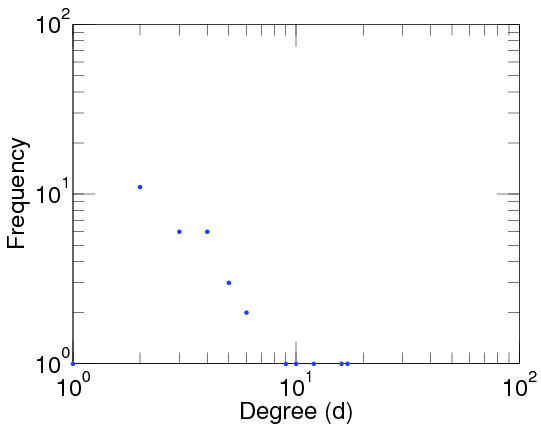
\includegraphics[width=65mm]{images/zachary_degree_dist.png} &   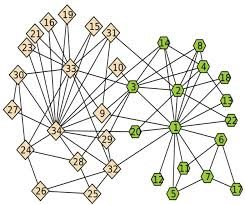
\includegraphics[width=65mm]{images/karate_true.png} \\
(a) Karate network degree distribution & (b) True communities of the karate network \\[6pt]
	\end{tabular}
	\caption{Degree distribution of the karate club network\cite{Kunegis2013}}
	\label{logo}
\end{figure}



\begin{figure}
	\begin{tabular}{cc}
		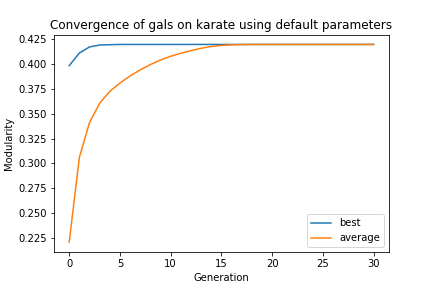
\includegraphics[width=65mm]{images/gals_default_karate.png} &   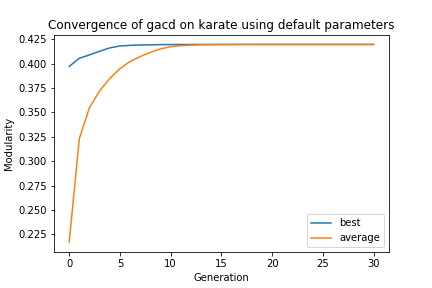
\includegraphics[width=65mm]{images/gacd_default_karate.png} \\
		(a) GALS & (b) GACD \\[6pt]
		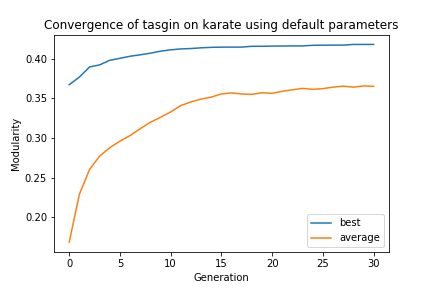
\includegraphics[width=65mm]{images/tasgin_default_karate.png}  &
		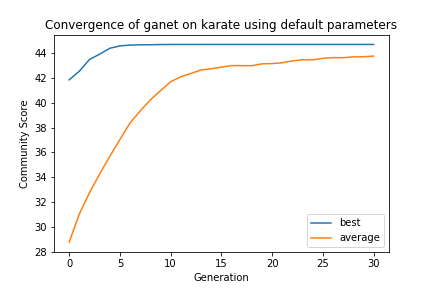
\includegraphics[width=65mm]{images/ganet_default_karate.png} \\
		(c) Tasgin & (d) GA-Net \\[6pt]
	\end{tabular}
	\caption{The average and best fitness, for each generation of the selected algorithms on 20  runs on the karate club network}
\end{figure}


\begin{figure}[!htb]
	\begin{center}
		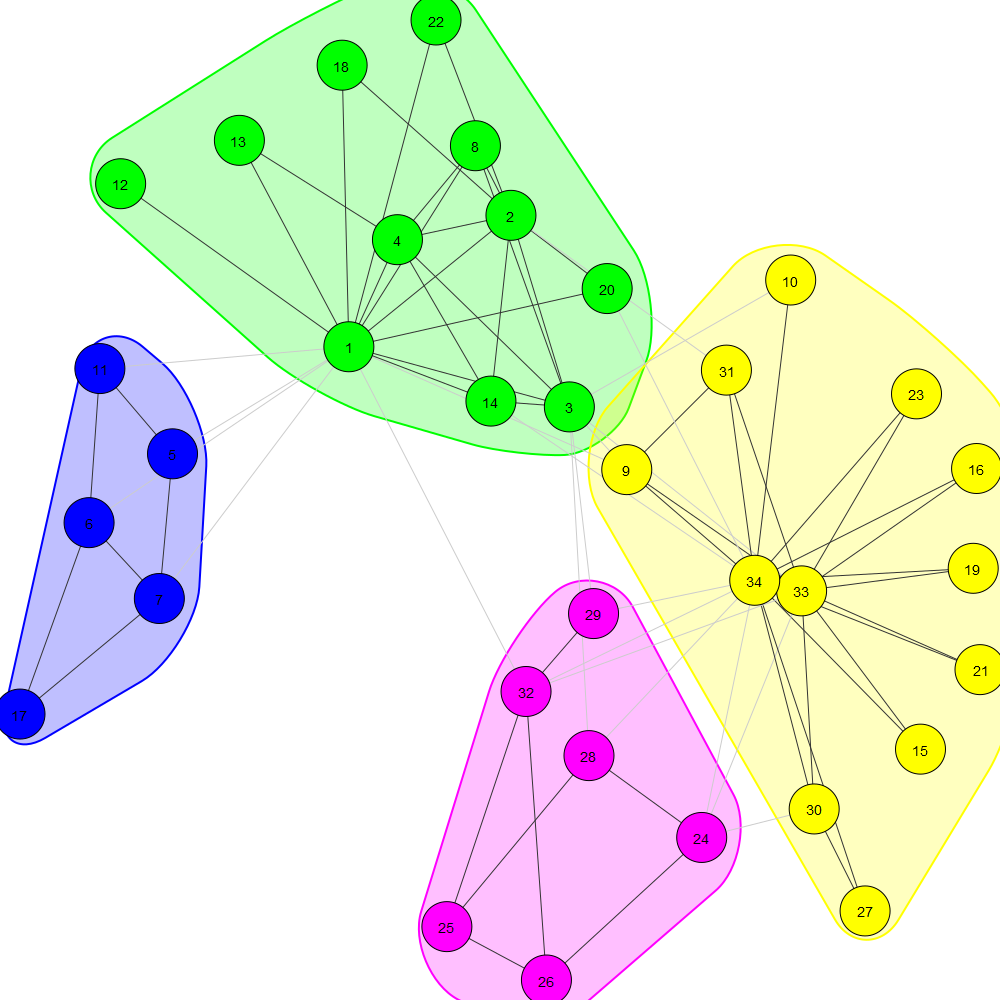
\includegraphics[scale=.2]{images/gals_karate_com.png} 
	\end{center}
	\caption{Community structure of the karate network discovered by GALS.}
	\label{logo}
\end{figure}


\subsection{Dolphins}
\cite{Lusseau2003}
\begin{figure}[!htb]
	\begin{center}
		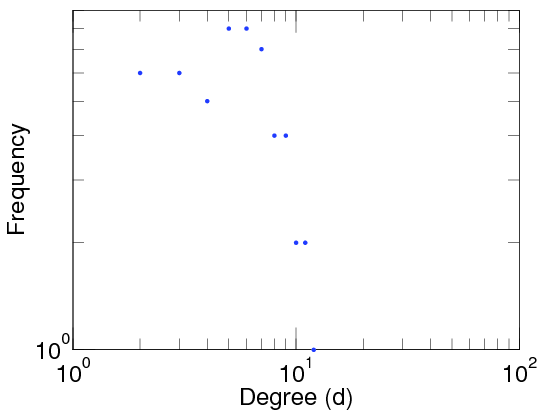
\includegraphics[scale=.4]{images/dolphins_degree_dist.png}
	\end{center}
	\caption{Degree distribution of the Dolphins network\cite{Kunegis2013}}
	\label{logo}
\end{figure}


\subsection{College Football}

\cite{Girvan2002}
\begin{figure}[!htb]
	\begin{center}
		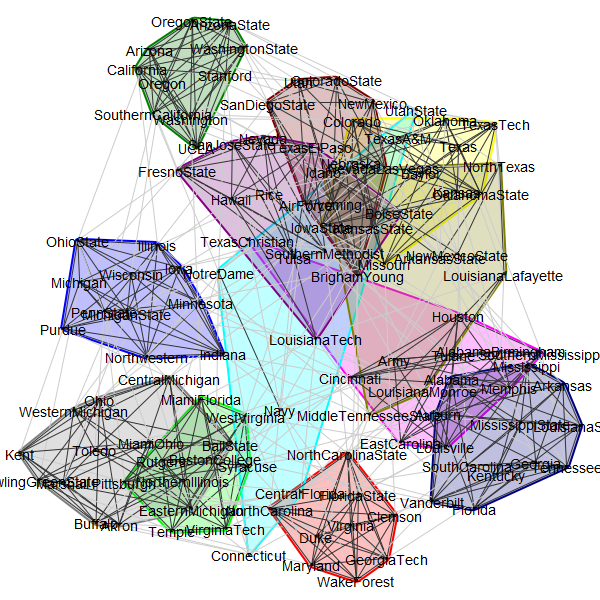
\includegraphics[scale=.4]{images/football.png}
	\end{center}
	\caption{The College Football network, with conferences grouped as communities}
	\label{logo}
\end{figure}


\subsection{Political Blogs}
While the experiments performed have been limited to undirected, unweighted networks, these GA approaches also apply to directed unweighted graphs with little change to the implementation. The Political blogs dataset\cite{Adamic2005} is an observed network, constructed from hyperlinks between blogs focusing on political topics. The data was collected during the course of the United States 2004 federal election campaign. Based on the content of each website, they have been hand labeled as leaning to the left or right of the political spectrum.
\begin{figure}
	\begin{tabular}{cc}
		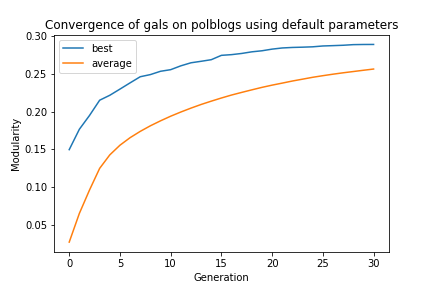
\includegraphics[width=65mm]{images/gals_default_polblogs.png} &   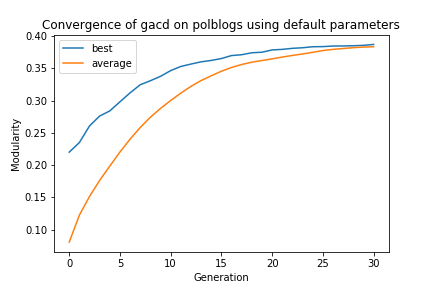
\includegraphics[width=65mm]{images/gacd_default_polblogs.png} \\
		(a) GALS & (b) GACD \\[6pt]
		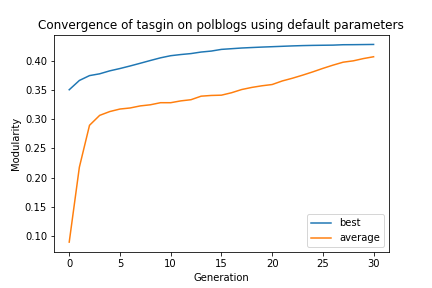
\includegraphics[width=65mm]{images/tasgin_default_polblogs.png}  &
		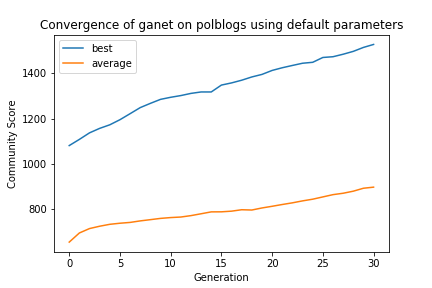
\includegraphics[width=65mm]{images/ganet_default_polblogs.png} \\
		(c) Tasgin & (d) GA-Net \\[6pt]
	\end{tabular}
	\caption{The average and best fitness, for each generation of the selected algorithms on 20  runs on the political blogs network}
\end{figure}


The network contains multiple disconnected components of only one node, as well as self-edges, or loops. While a generated network would not assign a single disconnected component a community membership that would be impossible to fulfill, the blogs with no connection to another are still labeled, and will adversely affect the results. For completeness, we present the outputs of both the original network, and a simplified version with no singleton nodes or self edges. 

\begin{figure}
	\begin{tabular}{cc}
		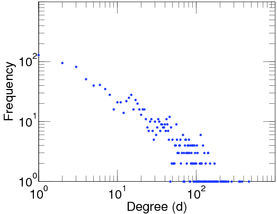
\includegraphics[width=65mm]{images/blogs_total.png} &   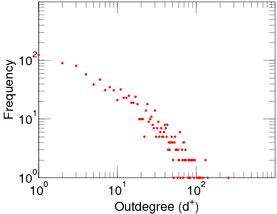
\includegraphics[width=65mm]{images/blogs_out.png} \\
		(a) Total Degree & (b) Outdegree \\[6pt]
		\multicolumn{2}{c}{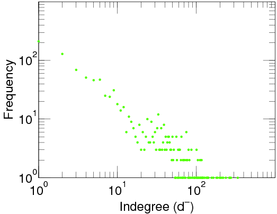
\includegraphics[width=65mm]{images/blogs_in.png} }\\
		\multicolumn{2}{c}{(c) Indegree}
	\end{tabular}
	\caption{The total degree, indegree and outdegree distribution for the political blogs network\cite{Kunegis2013}}
\end{figure}